%% ===================================================================
%%  CSE 402 -- Numerical Analysis, Simulation and Modeling Sessional
%%  Final report, ACM "acmart" sigconf template.
%%
%%  BUILD:   build.bat          (Windows)
%%           make               (make / latexmk)
%%           or manually:
%%           pdflatex main -> bibtex main -> pdflatex main -> pdflatex main
%%
%%  >>> EDIT THESE TWO LINES BEFORE SUBMITTING <<<
%% ===================================================================
\newcommand{\GROUPNUM}{02}                                  % <-- your group number
\newcommand{\REPOURL}{https://github.com/Ahnaf-Akib-Tanim/Numeric-Project-submission}  % <-- your public repo
%% ===================================================================

\documentclass[sigconf,nonacm]{acmart}

\usepackage{booktabs}
\usepackage{multirow}
\usepackage{amsmath}
% NB: do not load amssymb -- it clashes with acmart's newtx math setup
% ("Command \Bbbk already defined") and nothing here needs it.
\usepackage{graphicx}
\usepackage{algorithm}
\usepackage{algpseudocode}
\usepackage{xcolor}

% --- course report, not a real ACM submission --------------------------
\settopmatter{printacmref=false}
\renewcommand\footnotetextcopyrightpermission[1]{}
\pagestyle{plain}
\setcopyright{none}

\definecolor{hl}{HTML}{184F95}
\newcommand{\best}[1]{\textbf{#1}}

\begin{document}

\title{Discrete-Event Simulation and Constrained Optimisation of
       Emergency-Department Patient Flow}
% acmart's \subtitle takes plain text only -- no line breaks, no math.
\subtitle{A From-Scratch Replication of Lv et al. (2026) and Four Extensions}
\titlenote{CSE 402 --- Numerical Analysis, Simulation and Modeling Sessional.
           \textbf{Group \GROUPNUM, Section C.} Code and all generated results:
           \url{\REPOURL}}

\author{Sudip Kumar Saha}
\affiliation{%
  \institution{Student ID 2105152}
  \city{CSE}
  \country{BUET}}
\email{2105152@ugrad.cse.buet.ac.bd}

\author{Ahnaf Akib Tanim}
\affiliation{%
  \institution{Student ID 2105154}
  \city{CSE}
  \country{BUET}}
\email{2105154@ugrad.cse.buet.ac.bd}

\author{Md. Shahjalal Rumman}
\affiliation{%
  \institution{Student ID 2105165}
  \city{CSE}
  \country{BUET}}
\email{2105165@ugrad.cse.buet.ac.bd}

\author{Md. Dulal Hossain}
\affiliation{%
  \institution{Student ID 2105169}
  \city{CSE}
  \country{BUET}}
\email{2105169@ugrad.cse.buet.ac.bd}

\author{Md. Shoaib Hossain}
\affiliation{%
  \institution{Student ID 2105170}
  \city{CSE}
  \country{BUET}}
\email{2105170@ugrad.cse.buet.ac.bd}

\renewcommand{\shortauthors}{Saha, Tanim, Rumman, Hossain and Hossain
                             --- Group \GROUPNUM, Section C}

%% ======================================================================
\begin{abstract}
Emergency departments (EDs) must decide, every time a physician becomes free,
which of three competing queues to serve: newly arrived urgent patients, newly
arrived non-urgent patients, or patients returning for a follow-up after
diagnostics. We rebuild from scratch the discrete-event simulation (DES) of
Lv et al.\ (2026), which compares three physician-scheduling heuristics on a
Chinese tertiary-hospital ED, and validate it against every published KPI. We
then extend it in four directions the base paper does not attempt. First, we
add the c$\mu$ rule and its generalisation, scheduling policies that are
\emph{provably} optimal for a stated delay-cost objective rather than
hand-designed. Second, we replace the paper's two-stage brute-force grid search
over the slack thresholds $(k_1,k_2)$ with a hand-implemented Nelder--Mead
simplex driven by a sample-average approximation and an exterior penalty for
the service-level constraint. Third, we introduce an explicit weekly cost model
and jointly optimise the integer physician roster together with the thresholds.
Fourth, we apply exact common random numbers (CRN) and quantify the resulting
variance reduction. The rebuild reproduces all six structural findings of the
paper and its equipment-utilisation table to within $0.5$ percentage points,
although absolute waiting times run $12$--$25\%$ higher at the implied system
load $\rho\approx0.87$. Nelder--Mead matches the lattice optimum to $0.006$
minutes using $19\times$ fewer simulations; the cost-optimal roster saves
$20.7\%$ of weekly cost; CRN removes $98.9\%$ of comparison variance. Notably,
the paper's own published thresholds are infeasible on our model, which
motivates constrained re-tuning rather than parameter reuse.
\end{abstract}

\begin{CCSXML}
<ccs2012>
<concept>
<concept_id>10010405.10010481.10010487</concept_id>
<concept_desc>Applied computing~Health informatics</concept_desc>
<concept_significance>500</concept_significance>
</concept>
<concept>
<concept_id>10003752.10010070.10010071.10010261</concept_id>
<concept_desc>Theory of computation~Scheduling algorithms</concept_desc>
<concept_significance>500</concept_significance>
</concept>
<concept>
<concept_id>10010147.10010341.10010342.10010343</concept_id>
<concept_desc>Computing methodologies~Discrete-event simulation</concept_desc>
<concept_significance>500</concept_significance>
</concept>
<concept>
<concept_id>10002950.10003705.10011686</concept_id>
<concept_desc>Mathematics of computing~Nonconvex optimization</concept_desc>
<concept_significance>300</concept_significance>
</concept>
</ccs2012>
\end{CCSXML}

\ccsdesc[500]{Applied computing~Health informatics}
\ccsdesc[500]{Computing methodologies~Discrete-event simulation}
\ccsdesc[500]{Theory of computation~Scheduling algorithms}
\ccsdesc[300]{Mathematics of computing~Nonconvex optimization}

\keywords{discrete-event simulation, emergency department, patient scheduling,
          c$\mu$ rule, Nelder--Mead, simulation optimisation, common random
          numbers, variance reduction, staffing}

\maketitle

%% ======================================================================
\section{Introduction and Base Paper Review}

\subsection{Background}
Emergency departments are the classic congestion bottleneck of a hospital.
Demand is stochastic and strongly non-stationary, service is heterogeneous, and
the critical resource --- physician time --- is both scarce and expensive.
Because patients are triaged into urgency levels with different clinical
waiting targets, an ED is naturally modelled as a \emph{multi-class queue with
deadlines}. Simulation is the standard tool for evaluating operational policies
in this setting~\cite{vanbrabant2019kpi,wang2023simopt}, because the
combination of time-varying arrival rates, non-exponential service and
history-dependent priority rules puts exact analytic treatment out of
reach~\cite{huang2015control}.

\subsection{The base paper}
Our base paper is Lv, Liu, Yan and Wang~\cite{lv2026des}. It constructs a DES of
a Grade-A tertiary-hospital ED in China restricted to triage Level~III (urgent)
and Level~IV (non-urgent) patients, who together account for the great majority
of ED visits. Each patient arrives according to a non-homogeneous Poisson
process whose rate $\lambda_{d,h}$ varies by day and hour, waits for an
\emph{initial} consultation, may then require diagnostics (laboratory, X-ray,
CT or B-ultrasound), and if so returns to compete for the same physicians in a
\emph{follow-up} queue. Physicians work three shifts per day staffed
$(5,5,3)$.

The paper's contribution is to compare three physician-scheduling policies
within one unified simulation framework:

\begin{itemize}
\item \textbf{Initial-First (IFP)}: new arrivals always take precedence, Level
      III before Level IV, and follow-ups are served only with leftover
      capacity.
\item \textbf{Alternating 1:1 (ALT)}: at most half the physicians may work on
      initial consultations at any time; the remainder take follow-ups.
\item \textbf{Slack-Based (SBP)}: a patient of level $\ell$ is flagged
      \emph{urgent} once their waiting time reaches $T_\ell - k_\ell$, where
      $T_\ell$ is the triage target and $k_\ell$ is a tunable slack
      parameter~\cite{davenport2001slack}. Priority is then
      urgent-L3 $>$ urgent-L4 $>$ follow-up $>$ non-urgent initial.
\end{itemize}

SBP's thresholds are tuned by a two-stage brute-force grid search (coarse step
$1.0$, then fine step $0.1$), yielding $(k_1,k_2)=(13.1,2.1)$ and a reported
reduction in mean waiting time from $46.26$~min (IFP) to $35.25$~min, i.e.\
$23.8\%$, with no service-level violations. Statistical significance is
established with paired $t$-tests, a Bonferroni correction and Cohen's $d$.

\subsection{Gaps and objectives}
The base paper is a well-constructed comparison, but it leaves four concrete
openings, summarised in Table~\ref{tab:gaps}. Neither its source code nor its
operational dataset is public; only summary statistics are published, which is
nevertheless sufficient to rebuild an equivalent simulator.

\begin{table}[t]
\caption{Gaps in the base paper and the corresponding contribution of this work.}
\label{tab:gaps}
\small
\begin{tabular}{@{}p{2.9cm}p{2.9cm}p{1.6cm}@{}}
\toprule
\textbf{Paper does} & \textbf{Paper does not} & \textbf{Our work} \\
\midrule
Grid-search two thresholds & Optimise the \emph{staffing level} jointly & \S\ref{sec:cost} \\
Compare three heuristics & Compare against a provably optimal rule & \S\ref{sec:cmu} \\
Brute-force search & Use a derivative-free numerical optimiser & \S\ref{sec:opt} \\
100 independent replications & Apply variance reduction & \S\ref{sec:crn} \\
Report results & Release engine or data & \S\ref{sec:impl} \\
\bottomrule
\end{tabular}
\end{table}

Accordingly the objectives of this work are: (i)~to rebuild the model from
scratch and establish how faithfully the published results can be reproduced
from the published parameters alone; (ii)~to introduce a scheduling rule
derived from queueing theory rather than designed by hand; (iii)~to replace
brute-force tuning with a genuine numerical optimiser under an explicit
constraint, and to measure the efficiency gain in a hardware-independent way;
(iv)~to answer the staffing question the paper only probes by sensitivity
analysis; and (v)~to sharpen the statistical comparison through variance
reduction.

%% ======================================================================
\section{Methodology}

\subsection{System model}
Let $t$ denote simulated time in minutes over a horizon of one operational week
($T=10{,}080$). Following the paper, the day and hour indices are
\begin{equation}
d = \left\lfloor \tfrac{t}{1440} \right\rfloor \bmod 7,
\qquad
h = \left\lfloor \tfrac{t \bmod 1440}{60} \right\rfloor ,
\end{equation}
so the arrival intensity $\lambda_{d,h}$ is piecewise constant with a weekly
cycle. Each arrival is assigned triage level $\ell\in\{3,4\}$ with
probabilities $0.25$ and $0.75$ and inherits the clinical waiting target
$T_3=30$, $T_4=120$ minutes. The state is three FIFO queues,
$W^t_{\text{init},3}$, $W^t_{\text{init},4}$ and $W^t_{\text{follow}}$,
competing for $R^t$ physicians.

\subsection{Discrete-event engine}
The simulator is a hand-written event loop over a binary min-heap; no
process-oriented simulation library is used, so every mechanism described in
the paper is explicit in the code. Events are 4-tuples
$(\textit{time},\textit{type},\textit{seq},\textit{payload})$ ordered
lexicographically; the monotone counter \textit{seq} makes the ordering total
and therefore the replication bit-for-bit reproducible. Five event types are
processed: shift change, arrival, consultation end, examination device release
and examination results ready. After every event a single \textsc{Dispatch}
routine is invoked, and \emph{that} is the only point at which the scheduling
policy acts (Algorithm~\ref{alg:loop}). Swapping a policy therefore changes no
other line of the simulator, which makes the comparison structurally fair.

\begin{algorithm}[t]
\caption{Discrete-event main loop}
\label{alg:loop}
\begin{algorithmic}[1]
\State push all arrivals and shift changes onto the heap $H$
\While{$H \neq \emptyset$}
  \State $e \gets \textsc{PopMin}(H)$
  \If{$e.\textit{time} \ge T$} \textbf{break} \EndIf
  \State $\textit{now} \gets e.\textit{time}$; accrue utilisation integrals
  \State apply the state transition of $e$
  \State $R \gets \textsc{FreePhysicians}(\textit{now})$
  \If{$R>0$ and some queue is non-empty}
    \State $P \gets \textsc{Policy.Allocate}(\textit{state},\textit{now},R)$
    \State start service for every patient in $P$
  \EndIf
\EndWhile
\end{algorithmic}
\end{algorithm}

Service is non-preemptive: when a shift shrinks at 22:00 no consultation is
interrupted; the roster simply blocks new starts until the busy count falls
back below capacity.

\subsection{Arrival generation by thinning}
Because $\lambda(t)$ is a 168-piece step function, inverting its cumulative
intensity is error-prone. We instead sample the non-homogeneous Poisson process
by Lewis--Shedler thinning~\cite{lewis1979thinning}: with
$\lambda^{*}=\max_{d,h}\lambda_{d,h}=23.05$/h, generate a homogeneous process of
rate $\lambda^{*}$ by summing $\mathrm{Exp}(1/\lambda^{*})$ gaps and retain each
candidate epoch $t$ with probability $\lambda(t)/\lambda^{*}$. In an
infinitesimal interval a point is produced with probability
$\lambda^{*}\,\mathrm{d}t$ and survives with probability
$\lambda(t)/\lambda^{*}$, so the retained process has intensity
$\lambda(t)$ exactly. The acceptance rate is $\approx 58\%$.

\subsection{Service times by inverse-CDF sampling}
Consultation times are truncated exponentials $\mathrm{TruncExp}(\lambda_k,
[a_k,b_k])$. Inverting the truncated CDF gives
\begin{equation}
x = -\frac{1}{\lambda}
    \ln\!\left( e^{-\lambda a} - u\,(e^{-\lambda a}-e^{-\lambda b}) \right),
\qquad u\sim U(0,1),
\label{eq:truncexp}
\end{equation}
which consumes \emph{exactly one} uniform per variate. This is a deliberate
choice: rejection sampling would consume a variable number and would destroy
the stream synchronisation on which \S\ref{sec:crn} depends. The realised mean
after truncation follows in closed form,
\begin{equation}
\mathbb{E}[X] = a + \frac{1}{\lambda}
  - \frac{(b-a)\,e^{-\lambda(b-a)}}{1-e^{-\lambda(b-a)}} ,
\label{eq:truncmean}
\end{equation}
giving $9.093$~min for initial and $12.841$~min for follow-up consultations.
We note that a truncated exponential on $[5,25]$ \emph{cannot} attain a mean of
$15$~min --- $15$ is its supremum, approached only as $\lambda\to0$ --- so
$\lambda_2=1/15$ is the only reading of the paper consistent with its own
stated bounds, and it is the reading that reproduces the reported
$\approx85\%$ physician utilisation.

\subsection{Scheduling policies}
\label{sec:cmu}
IFP, ALT and SBP are implemented directly from Equations (8)--(23) of the base
paper. To these we add two policies derived from queueing theory.

\paragraph{The c$\mu$ rule (WSEPT).}
Cox and Smith~\cite{cox1961queues}, with the modern proof due to Buyukkoc et
al.~\cite{buyukkoc1985cmu}, show that for a multi-class queue served by a single
pool under \emph{linear} holding costs $c_\ell$ per unit waiting time, the
policy minimising expected total holding cost always serves the non-empty class
maximising the index
\begin{equation}
I_\ell = c_\ell\,\mu_\ell ,
\qquad \mu_\ell = 1/\mathbb{E}[S_\ell] .
\label{eq:cmu}
\end{equation}
We set $c_\ell = 1/T_\ell$: a minute of waiting hurts in inverse proportion to
how much waiting that class tolerates, which converts the triage targets
directly into delay costs. The resulting indices are given in
Table~\ref{tab:cmu}. This rule is also known as Weighted Shortest Expected
Processing Time. Crucially, its indices are \emph{constants}, so the classical
rule degenerates to a fixed priority order (L3 initial $>$ follow-up $>$ L4
initial). That is a genuine property of the theorem, and it is exactly the
limitation the generalisation removes.

\paragraph{The generalised c$\mu$ rule (Gc$\mu$).}
For \emph{convex} delay costs $C_\ell(w)$, Van Mieghem~\cite{vanmieghem1995gcmu}
and Mandelbaum and Stolyar~\cite{mandelbaum2004convex} show the asymptotically
optimal index is $C_\ell'(w)\,\mu_\ell$ evaluated at the head-of-line delay.
Taking $C_\ell(w)=(w/T_\ell)^2$ gives
\begin{equation}
I_\ell(t) = \frac{2\,w_{\text{head}}\,\mu_\ell}{T_\ell^{2}} ,
\label{eq:gcmu}
\end{equation}
which grows with how long the front patient has already waited. Gc$\mu$ is
therefore delay-adaptive like SBP, but it is \emph{derived} rather than tuned
and has no free parameters at all.

\begin{table}[t]
\caption{Index values computed by the c$\mu$ and generalised c$\mu$ rules under
         the base paper's parameters.}
\label{tab:cmu}
\small
\begin{tabular}{@{}lrrrr@{}}
\toprule
\textbf{Class} & $T_\ell$ & $\mathbb{E}[S_\ell]$ & $c_\ell$ & $\mathbf{c_\ell\mu_\ell}$ \\
\midrule
Level III initial & 30  & 9.093  & 0.03333 & \best{0.003666} \\
Follow-up         & 60  & 12.841 & 0.01667 & \best{0.001298} \\
Level IV initial  & 120 & 9.093  & 0.00833 & \best{0.000916} \\
\bottomrule
\end{tabular}
\end{table}

\paragraph{A fair objective.}
The c$\mu$ rule is optimal for the holding cost, not for the unweighted mean
wait, so judging it on the latter alone would be a category error. We therefore
also report the \emph{holding cost}
\begin{equation}
H = \frac{1}{N}\sum_{i=1}^{N} \frac{w_i}{T_{\ell(i)}} ,
\label{eq:holding}
\end{equation}
i.e.\ waiting measured in units of each patient's own clinical tolerance.

\subsection{Constrained simulation optimisation}
\label{sec:opt}
The tuning problem of the base paper is
\begin{equation}
\min_{k_1,k_2}\ \overline{W}_{\text{total}}(k_1,k_2)
\quad \text{s.t.} \quad SL_\ell(k_1,k_2) \ge SL^{\min}_\ell,\ \ell\in\{3,4\}.
\label{eq:problem}
\end{equation}
Three ingredients turn this into something a simplex method can solve.

\paragraph{Sample average approximation.}
A simulation objective is random, and simplex methods stall on noisy surfaces.
We minimise instead the sample average over a \emph{fixed} set of $n$ patient
streams~\cite{kim2015saa}. Because the engine is deterministic given a stream,
$\hat{F}$ is a genuine deterministic function: evaluating the same point twice
returns the identical value. The common seeds also cancel between candidates,
which smooths the surface far below the pointwise noise level.

\paragraph{Exterior penalty.}
Nelder--Mead is unconstrained, so the service-level constraint is folded in as
\begin{equation}
F(k_1,k_2) = \overline{W}_{\text{total}}
 + \mu \sum_{\ell\in\{3,4\}} \max\!\left(0,\ SL^{\min}_\ell - SL_\ell\right),
\label{eq:penalty}
\end{equation}
with $\mu = 500$ minutes per unit of shortfall: one percentage point of
service-level shortfall costs as much as five extra minutes of average
waiting~\cite{nocedal2006numerical}. This is large enough that an infeasible
point is never optimal, yet small enough that the penalised surface remains
smooth near the boundary. Box bounds $k\ge0$ are enforced by
\emph{projection}, so the simplex can slide along a bound rather than being
repelled from it.

\paragraph{Nelder--Mead.}
We implement the downhill simplex method~\cite{nelder1965simplex} from scratch
(Algorithm~\ref{alg:nm}) with the standard coefficients $\alpha=1$, $\gamma=2$,
$\rho=0.5$, $\sigma=0.5$. Two details matter in practice. The initial simplex
uses a \emph{per-dimension} step $(4,15)$, because $k_1$ lives on $\approx[0,30]$
against $T_3=30$ while $k_2$ lives on $\approx[0,120]$ against $T_4=120$; a
single scalar step would produce a badly conditioned simplex. Second, since the
method is local, we run it from four dispersed starts and report the spread.

\begin{algorithm}[t]
\caption{Nelder--Mead iteration (minimisation)}
\label{alg:nm}
\begin{algorithmic}[1]
\State order vertices so that $f(x_1)\le\cdots\le f(x_{n+1})$
\State \textbf{stop} if simplex span $\le x_{\text{tol}}$ and
       $f(x_{n+1})-f(x_1)\le f_{\text{tol}}$
\State $x_c \gets \frac{1}{n}\sum_{i\le n} x_i$ \Comment{centroid without worst}
\State $x_r \gets \Pi\!\left(x_c + \alpha (x_c - x_{n+1})\right)$ \Comment{reflect}
\If{$f(x_r) < f(x_1)$}
  \State $x_e \gets \Pi\!\left(x_c + \gamma (x_r - x_c)\right)$ \Comment{expand}
  \State $x_{n+1} \gets \arg\min\{f(x_e),f(x_r)\}$
\ElsIf{$f(x_r) < f(x_n)$}
  \State $x_{n+1} \gets x_r$
\Else
  \State $x_k \gets \Pi\!\left(x_c + \rho\,(\cdot - x_c)\right)$ \Comment{contract}
  \If{improved} $x_{n+1} \gets x_k$
  \Else\ $x_i \gets \Pi\!\left(x_1 + \sigma (x_i - x_1)\right)\ \forall i>1$
  \EndIf
\EndIf
\end{algorithmic}
\end{algorithm}

Here $\Pi(\cdot)$ denotes projection onto the box. The optimiser's cost is
counted in \emph{week-long simulations}, not seconds, so the comparison against
the paper's lattice is independent of hardware and of the degree of
parallelism.

\subsection{Cost-based staffing}
\label{sec:cost}
The paper varies staffing but cannot recommend a level, because it has no way
to price a physician-hour against a patient-waiting-minute. We supply the
missing objective:
\begin{equation}
C(R,k_1,k_2) = \alpha H_{\text{phys}} + \beta W_{\text{total}}
             + \gamma V_{\text{SLA}} ,
\label{eq:cost}
\end{equation}
where $R=(R_{\text{m}},R_{\text{a}},R_{\text{n}})$ is the integer roster,
$H_{\text{phys}}$ is rostered physician-hours per week, $W_{\text{total}}$ is
total patient waiting-minutes per week and $V_{\text{SLA}}$ counts patients
past their triage target. Because the best thresholds for a 3-physician night
shift are not the best for a 5-physician one, $(k_1,k_2)$ is \emph{re-optimised
inside every candidate roster}, making this a joint rather than a sequential
optimisation. The search is two-stage: all rosters in $\{2,\dots,8\}^3$ (minus
those staffing nights above days) are screened cheaply and unstable ones ---
where more than $15\%$ of the week's patients remain in system at the horizon,
so the queue is growing rather than clearing --- are discarded; the best
candidates then receive a full Nelder--Mead re-tune.

\subsection{Common random numbers and inference}
\label{sec:crn}
For two policies $A$ and $B$,
\begin{equation}
\operatorname{Var}(A-B) = \operatorname{Var}(A) + \operatorname{Var}(B)
                        - 2\operatorname{Cov}(A,B).
\label{eq:crn}
\end{equation}
Independent streams give $\operatorname{Cov}=0$. Under CRN both policies face
the identical simulated week, so a heavy week inflates both together,
$\operatorname{Cov}$ becomes strongly positive and the variance of the
\emph{difference} collapses while each marginal variance is
unchanged~\cite{law2015simulation}.

Most implementations forfeit much of this benefit through desynchronisation:
once two policies diverge they consume random numbers in a different order. We
avoid it structurally. Six independent PCG64 substreams~\cite{oneill2014pcg}
are spawned from one seed (arrivals, triage levels, initial service, follow-up
service, examination need, examination selection); the \emph{entire} exogenous
patient stream --- arrival times, levels, both consultation durations,
diagnostics required --- is materialised \emph{before} the run starts, so the
engine draws no random number while simulating; and each variate consumes
exactly one uniform by Eq.~\eqref{eq:truncexp}. Patient $\#1723$ is therefore
bit-identical under every policy.

Inference follows the base paper: paired $t$-tests on the per-replication means
(paired, because CRN makes the design paired), a Bonferroni correction across
the comparison family, and Cohen's $d$ in its paired form
$\bar{d}/s_d$. We additionally report the smallest $n$ satisfying
$t_{0.975,n-1}\,s/\sqrt{n} \le h$, solved by iteration since the $t$ quantile
itself depends on $n$.

%% ======================================================================
\section{Implementation and Experiments}
\label{sec:impl}

\subsection{Software}
The simulator is implemented in Python 3.11 in approximately $7{,}900$ lines
across a $15$-module library, $10$ runnable experiment scripts and a
$33$-check verification suite. Only NumPy~\cite{harris2020numpy},
SciPy~\cite{virtanen2020scipy}, Matplotlib~\cite{hunter2007matplotlib} and
pandas are used; SciPy appears only for distribution quantiles, the
$t$-distribution, and as a deliberate cross-check of our own optimiser. The
library preserves the five-module architecture of the base paper's Figure~2 so
that code and paper can be read side by side: entity definition, event
scheduling, resource scheduling, strategy execution and statistical output.
The complete code is available at \url{\REPOURL}.

One implementation note has a material effect. Events were initially an ordered
dataclass; profiling showed Python-level comparisons in the heap consumed $22\%$
of runtime. Replacing them with plain tuples moved comparison into C and cut
per-replication time from $0.20$\,s to $0.076$\,s --- which is what makes the
$50{,}415$-simulation grid search of \S\ref{sec:resopt} affordable at all.

\subsection{Parameters}
All parameters are taken from the base paper and are listed in
Table~\ref{tab:params}. Arrival rates are its Table~2 verbatim ($7\times24$
values). The analytic offered load implied by these parameters is
\begin{equation}
\rho = \frac{N\left(\mathbb{E}[S_1] + p_{\text{exam}}\mathbb{E}[S_2]\right)}
            {\sum_{s} L_s R_s \cdot 7} = 0.870 ,
\end{equation}
consistent with the $84.98$--$85.43\%$ physician utilisation the paper reports,
which confirms the parameterisation before any simulation is run.

\begin{table}[t]
\caption{Model parameters. All values are from the base paper except the five
         marked $^\dagger$, which it does not specify.}
\label{tab:params}
\small
\begin{tabular}{@{}p{3.6cm}p{4.0cm}@{}}
\toprule
\textbf{Parameter} & \textbf{Value} \\
\midrule
Horizon / replications      & 10{,}080 min (1 week) / 100 \\
Arrival rate $\lambda_{d,h}$& Table 2, $7\times24$; peak 23.05/h \\
Triage mix                  & 25\% Level III, 75\% Level IV \\
Targets $T_3$, $T_4$        & 30 min, 120 min \\
Initial consultation        & TruncExp$(1/9)$ on $[5,15]$ \\
Follow-up consultation      & TruncExp$(1/15)$ on $[5,25]$ \\
$P(\text{diagnostics})$     & 0.60 \\
Modality probabilities      & Lab .92, CT .55, X-ray .29, US .22 \\
Modality durations          & 1.19, 2.45, 3.99, 6.58 min \\
Report delays               & 20, 30, 30, 0 min \\
Shifts (M/A/N)              & 5 / 5 / 3 physicians \\
\midrule
$SL^{\min}_\ell$            & $0.95^\dagger$ \\
$T_{\text{follow}}$ (c$\mu$)& $60$ min$^\dagger$ \\
Search box                  & $k_1\in[0,30]$, $k_2\in[0,60]^\dagger$ \\
Cost weights $\alpha,\beta,\gamma$ & $120$, $0.50$, $50^\dagger$ \\
``At least one'' exam rule  & resample$^\dagger$ \\
\midrule
Base seed                   & 20250402 \\
\bottomrule
\end{tabular}
\end{table}

\subsection{Parameters we had to choose}
The paper leaves exactly five quantities unspecified. $SL^{\min}_\ell$ is
written as a constraint but never given a number; we use $0.95$, a standard ED
target, strict enough that the penalty binds. $T_{\text{follow}}$, needed by the
c$\mu$ rule, is set to $60$~min, the midpoint of $T_3$ and $T_4$; a sweep from
$15$ to $120$~min leaves the policy ranking unchanged. The search box must at
least contain the paper's own reported winners at $k_1=26$ and $k_2=40$. The
cost weights exist only in our extension and are stress-tested in
\S\ref{sec:resstaff}. Finally, the paper states that $60\%$ of patients need
``at least one'' test while also giving independent per-modality probabilities
that jointly select none with probability $1.99\%$; we resample so that ``at
least one'' holds exactly.

\subsection{Experimental design}
Every comparison uses $100$ replications of one simulated week per policy under
CRN, matching the base paper's replication count. Replication $r$ of every
policy uses the identical patient stream, so all comparisons are exactly
paired. Experiments were executed on a 16-core machine with 14 worker
processes; the complete pipeline runs in about $20$ minutes, of which the
brute-force grid search is roughly half.

\subsection{Verification}
Correctness is checked by 33 automated assertions, each pinning down a property
that some reported number depends on: the samplers against their closed forms
(Eq.~\eqref{eq:truncmean} against $200{,}000$ draws), the day/hour indexing,
convergence of the thinned arrival process, CRN seed behaviour, and engine
invariants --- no patient served before arrival, no idle physician while a
patient waits (work conservation, verified for every policy), the sequential
examination chain, and non-preemptive shift changes. The optimiser is checked
against the Rosenbrock function and against SciPy. All 33 pass.

%% ======================================================================
\section{Results and Discussion}

\subsection{Model validation}
Figure~\ref{fig:arrivals} confirms the input process: over $200$ sampled weeks
the realised hourly arrival counts reproduce the paper's Table~2 with a
relative $L_1$ error of $1.67\%$ and correlation $0.9991$.

\begin{figure}[t]
\centering
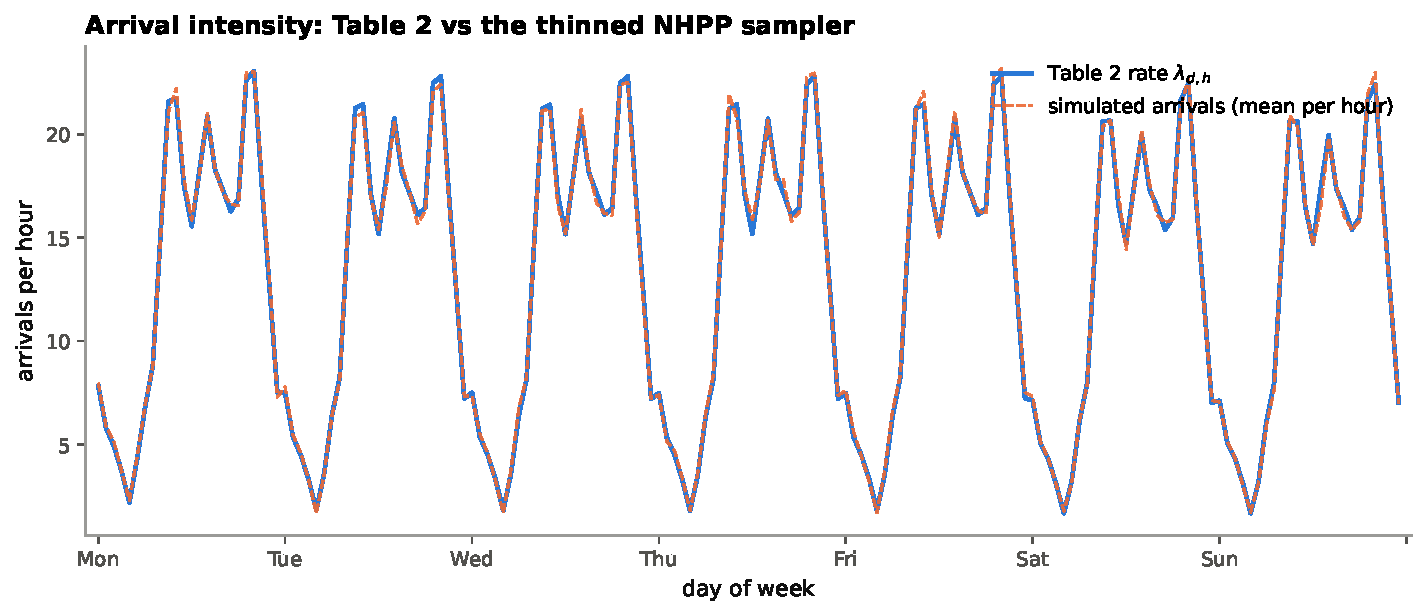
\includegraphics[width=\columnwidth]{figures/wp1_arrival_validation.pdf}
\caption{Validation of the thinned non-homogeneous Poisson arrival process
         against the base paper's published hourly rates.}
\Description{Two overlapping curves of arrivals per hour across a week; the
simulated curve tracks the published rate curve almost exactly across all
168 hourly bins.}
\label{fig:arrivals}
\end{figure}

Table~\ref{tab:validate} compares every published KPI. The agreement is
structural rather than numerical. Reproduced closely: both service levels under
IFP ($100\%/100\%$), ALT's Level III waiting time ($6.05$ vs.\ $6.82$
published), SBP's Level III waiting time ($12.35$ vs.\ $10.48$), physician
utilisation ($86.3\%$ vs.\ $85.0$--$85.4\%$) and its near-invariance across
policies, and --- strikingly --- the equipment-utilisation table
(Table~\ref{tab:equip}), which matches within $0.5$ percentage points on all
four modalities. This reproduces the paper's central managerial conclusion that
physicians, not equipment, are the bottleneck.

\begin{table}[t]
\caption{Validation against the base paper. Deviation is relative to the
         published value; $100$ replications.}
\label{tab:validate}
\small
\begin{tabular}{@{}llrrr@{}}
\toprule
\textbf{Policy} & \textbf{Metric} & \textbf{Ours} & \textbf{Paper} & \textbf{Dev.} \\
\midrule
\multirow{4}{*}{IFP}
 & Mean wait, all (min)   & 52.43  & 46.26  & $+13.3\%$ \\
 & Mean wait, Level III   & 50.88  & 44.14  & $+15.3\%$ \\
 & Service level L3 / L4  & 100 / 100 & 100 / 100 & $0.0\%$ \\
 & Physician utilisation  & 86.36  & 85.43  & $+1.1\%$ \\
\midrule
\multirow{4}{*}{ALT}
 & Mean wait, all (min)   & 42.39  & 37.88  & $+11.9\%$ \\
 & Mean wait, Level III   & 6.05   & 6.82   & $-11.2\%$ \\
 & Service level L3 / L4  & 99.96 / 87.37 & 98.08 / 89.29 & $-2.2\%$ \\
 & Physician utilisation  & 86.34  & 85.41  & $+1.1\%$ \\
\midrule
\multirow{4}{*}{SBP}
 & Mean wait, all (min)   & 44.08  & 35.25  & $+25.1\%$ \\
 & Mean wait, Level III   & 12.35  & 10.48  & $+17.9\%$ \\
 & Service level L3 / L4  & 99.99 / 89.40 & 100 / 100 & $-10.6\%$ \\
 & Physician utilisation  & 86.34  & 84.98  & $+1.6\%$ \\
\bottomrule
\end{tabular}
\end{table}

\begin{table}[t]
\caption{Diagnostic equipment utilisation, reproduced from the base paper's
         Table 9.}
\label{tab:equip}
\small
\begin{tabular}{@{}lrrr@{}}
\toprule
\textbf{Equipment} & \textbf{Exams/week} & \textbf{Ours} & \textbf{Paper} \\
\midrule
Laboratory   & 1248 & 14.73\% & 14.36\% \\
X-ray        &  394 & 15.59\% & 15.20\% \\
CT           &  748 & 18.18\% & 17.64\% \\
B-ultrasound &  297 & 19.41\% & 19.03\% \\
\bottomrule
\end{tabular}
\end{table}

What does \emph{not} reproduce is the absolute level: our waiting times run
$12$--$25\%$ higher. The explanation is a single number. The published
parameters imply $\rho\approx0.870$, and near saturation the mean wait is
hypersensitive to the last percentage point of utilisation, so a small
mismatch in the unrecoverable patient mix produces a large mismatch in waiting
time. Since the underlying dataset is not public, an exact numerical match is
not attainable and we do not claim one; we report the deviation openly rather
than tuning parameters to hit the published figure.

\subsection{Policy comparison}
Table~\ref{tab:master} is the consolidated comparison of all six policies, and
Figure~\ref{fig:tradeoff} is its geometric summary. WSEPT attains the lowest
holding cost ($0.3763$ against IFP's $0.7550$, a $50\%$ reduction), exactly as
the Cox--Smith result predicts, and on this system it also attains the lowest
unweighted mean wait ($42.32$~min). All differences against the paper's three
heuristics are significant after Bonferroni correction
(Table~\ref{tab:cmusig}).

\begin{table*}[t]
\caption{Consolidated comparison of all six scheduling policies; $100$
         common-random-number replications. SBP$^{*}$ is the Slack-Based Policy
         with our constrained Nelder--Mead thresholds. ``Meets SLA'' requires
         $SL_\ell\ge95\%$ on \emph{both} triage levels.}
\label{tab:master}
\begin{tabular}{@{}llrlrrrrrrc@{}}
\toprule
\textbf{Policy} & \textbf{Origin} & \textbf{Wait (min)} & \textbf{95\% CI} &
\textbf{L-III} & \textbf{L-IV} & \textbf{Holding} &
\textbf{$SL_3$} & \textbf{$SL_4$} & \textbf{Util.} & \textbf{Meets SLA} \\
\midrule
IFP    & base paper                & 52.43 & [49.63, 55.22] & 50.88 & 52.94 & 0.7550 & 100.00\% & 100.00\% & 86.36\% & yes \\
ALT    & base paper                & 42.39 & [40.26, 44.51] & 6.05  & 54.61 & 0.3913 & 99.96\%  & 87.37\%  & 86.34\% & \textbf{no} \\
SBP    & base paper $(13.1,2.1)$   & 44.08 & [41.72, 46.44] & 12.35 & 54.74 & 0.4450 & 99.99\%  & 89.40\%  & 86.34\% & \textbf{no} \\
SBP$^{*}$ & \textbf{ours} $(2.31,8.37)$ & 44.18 & [41.81, 46.55] & 14.14 & 54.27 & 0.4570 & 95.42\%  & 95.64\%  & 86.34\% & \best{yes} \\
WSEPT  & \textbf{ours}, c$\mu$     & \best{42.32} & [40.21, 44.43] & 3.76 & 55.30 & \best{0.3763} & 100.00\% & 86.87\% & 86.34\% & \textbf{no} \\
Gc$\mu$& \textbf{ours}, gen.\ c$\mu$ & 44.05 & [41.81, 46.29] & 14.59 & 53.94 & 0.4588 & 100.00\% & 90.99\%  & 86.35\% & \textbf{no} \\
\bottomrule
\end{tabular}
\end{table*}

\begin{table}[t]
\caption{Paired $t$-tests on the holding cost, WSEPT against every other
         policy. Bonferroni-adjusted $\alpha = 0.00333$.}
\label{tab:cmusig}
\small
\begin{tabular}{@{}lrrrr@{}}
\toprule
\textbf{Comparison} & \textbf{Diff.} & $t$ & $p$ & \textbf{Cohen's $d$} \\
\midrule
IFP vs.\ WSEPT    & $+0.3786$ & 31.67  & $1.3\!\times\!10^{-53}$ & 3.17 \\
ALT vs.\ WSEPT    & $+0.0150$ & 36.54  & $2.9\!\times\!10^{-59}$ & 3.65 \\
SBP vs.\ WSEPT    & $+0.0686$ & 14.15  & $1.6\!\times\!10^{-25}$ & 1.42 \\
WSEPT vs.\ Gc$\mu$& $-0.0824$ & $-33.42$ & $1.0\!\times\!10^{-55}$ & $-3.34$ \\
\bottomrule
\end{tabular}
\end{table}

\begin{figure}[t]
\centering
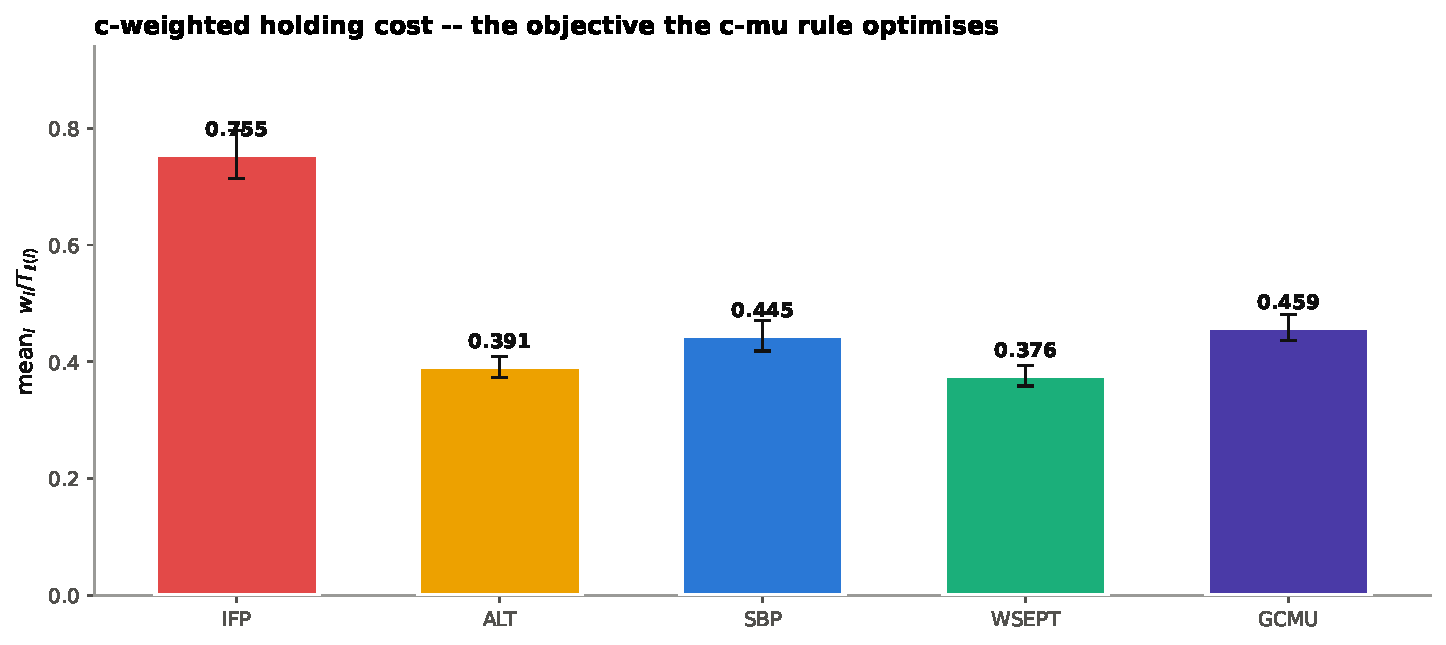
\includegraphics[width=\columnwidth]{figures/wp2_holding_cost_bars.pdf}
\caption{The objective the c$\mu$ rule is provably optimal for: waiting measured
         in units of each patient's own clinical tolerance
         (Eq.~\eqref{eq:holding}). Lower is better.}
\Description{Bar chart of holding cost by policy. IFP is about 0.755, roughly
twice every other policy; WSEPT is lowest at 0.376, followed by ALT, SBP and
generalised c-mu.}
\label{fig:holding}
\end{figure}

The service-level columns of Table~\ref{tab:master} carry the substantive
finding: \emph{the rules that sprint hardest on Level III are precisely the
rules that let Level IV breach}. WSEPT reaches only $86.9\%$ on Level IV, and
so do ALT and, importantly, the paper's own tuned SBP at $89.4\%$. Only IFP ---
which is slow --- and our re-tuned SBP$^{*}$ satisfy the constraint on both
levels. Consequently there is no single winner, and the honest answer depends
on the objective: WSEPT minimises both the holding cost and the raw mean wait;
SBP$^{*}$ is the fastest policy a hospital could actually adopt.

\begin{figure}[t]
\centering
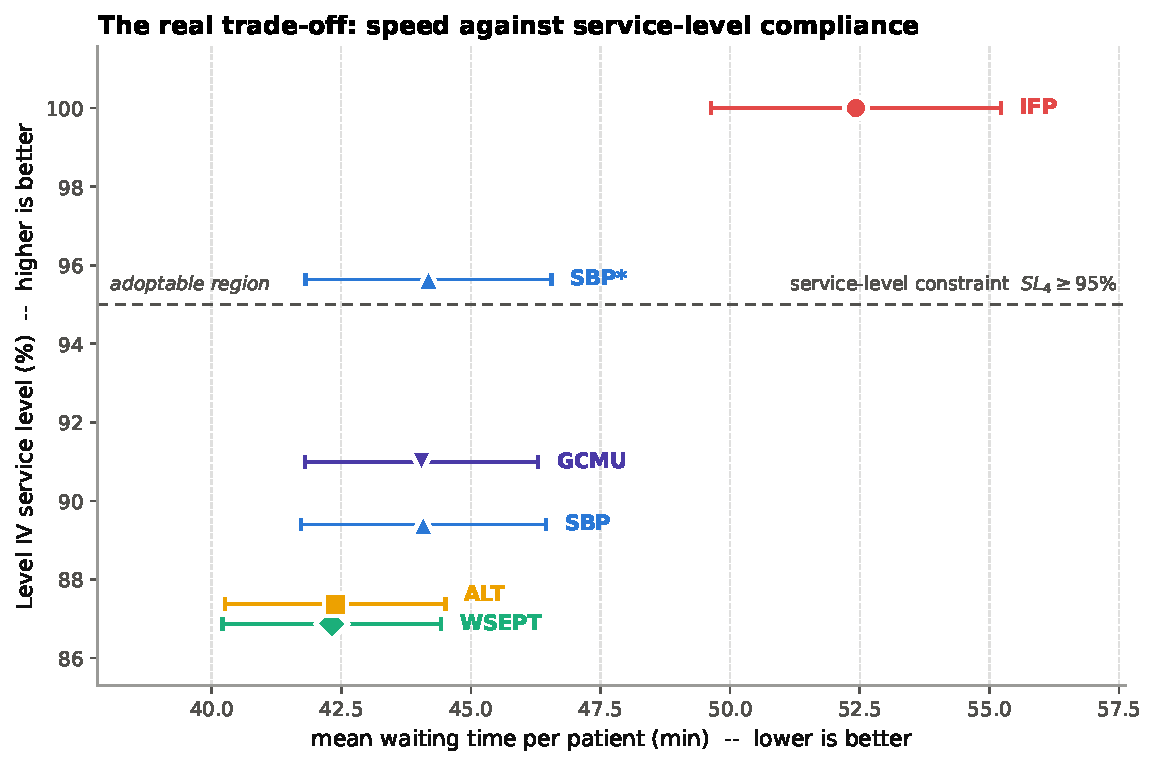
\includegraphics[width=\columnwidth]{figures/final_tradeoff.pdf}
\caption{Speed against service-level compliance. Only policies above the dashed
         constraint line are adoptable; of the tuned policies only SBP$^{*}$
         is both fast and feasible.}
\Description{Scatter plot with mean waiting time on the horizontal axis and
Level IV service level on the vertical axis. IFP sits top right, slow but at
100 percent. ALT, WSEPT, SBP and generalised c-mu sit bottom left, fast but
below the 95 percent dashed line. SBP star sits just above the line at about
44 minutes.}
\label{fig:tradeoff}
\end{figure}

We state one caveat explicitly. The Cox--Smith optimality proof assumes a
single-stage multi-class queue; our model has re-entrant flow, since patients
return for a follow-up after diagnostics, and a time-varying server pool.
The optimality guarantee is therefore approximate here, and we report the
empirical ranking rather than relying on the theorem.

\subsection{Optimiser versus brute force}
\label{sec:resopt}
Table~\ref{tab:budget} is the central efficiency result. Reproducing the paper's
procedure on our model, the two-stage lattice evaluated $2{,}332$ points at a
cost of $50{,}415$ week-long simulations --- roughly $970$ simulated
patient-years of ED operation --- to reach $(4.10,8.20)$. Our simplex reached
an equally good point in $2{,}650$ simulations, a $\mathbf{19.0\times}$
reduction. Re-scored afterwards on one identical full-length batch, the two
optima differ by $0.006$ minutes, far below the simulation's own noise floor.

\begin{table}[t]
\caption{Simulation budget required by brute-force grid search and by the
         hand-implemented Nelder--Mead simplex, on the identical objective and
         the identical patient streams.}
\label{tab:budget}
\small
\begin{tabular}{@{}lrrr@{}}
\toprule
\textbf{Method} & \textbf{Points} & \textbf{Simulations} & \textbf{Objective} \\
\midrule
Grid, coarse (step 1.0)  & 1{,}891 & 28{,}365 & 47.6105 \\
Grid, fine (step 0.1)    &    441  & 22{,}050 & 46.4601 \\
\textbf{Grid, total}     & 2{,}332 & \textbf{50{,}415} & 46.4601 \\
Nelder--Mead, 1 start    &     53  & \best{2{,}650} & 46.4668 \\
Nelder--Mead, 4 starts   &    196  & 9{,}800  & 46.4668 \\
\bottomrule
\end{tabular}
\end{table}

Four dispersed starts converge to objectives within $0.15$~min of one another
($46.468$--$46.622$), indicating an effectively unimodal penalised surface in
this box, and our implementation agrees with \texttt{scipy.optimize} to
$0.0000$~min on the same objective. Figure~\ref{fig:path} draws the simplex
trajectory on the very response surface the lattice had to evaluate
exhaustively; Figure~\ref{fig:conv} shows solution quality against budget.

\begin{figure}[t]
\centering
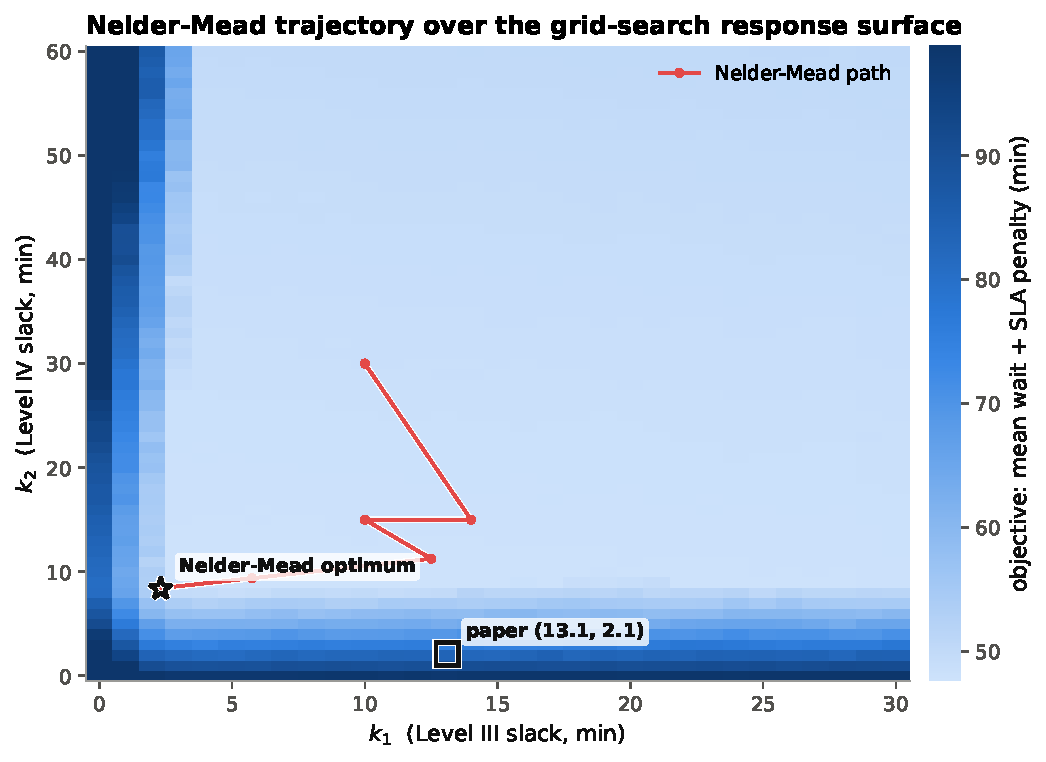
\includegraphics[width=\columnwidth]{figures/wp3_simplex_path.pdf}
\caption{The Nelder--Mead trajectory over the grid-search response surface. The
         dark band is the service-level penalty region; the base paper's
         published optimum (square) lies inside it.}
\Description{Heat map over k1 and k2 with a dark high-penalty band along the
bottom edge. A red path descends from the start point at (10, 30) to a star
marking the converged optimum near (2.3, 8.4). A square marks the paper
optimum at (13.1, 2.1) inside the dark band.}
\label{fig:path}
\end{figure}

\begin{figure}[t]
\centering
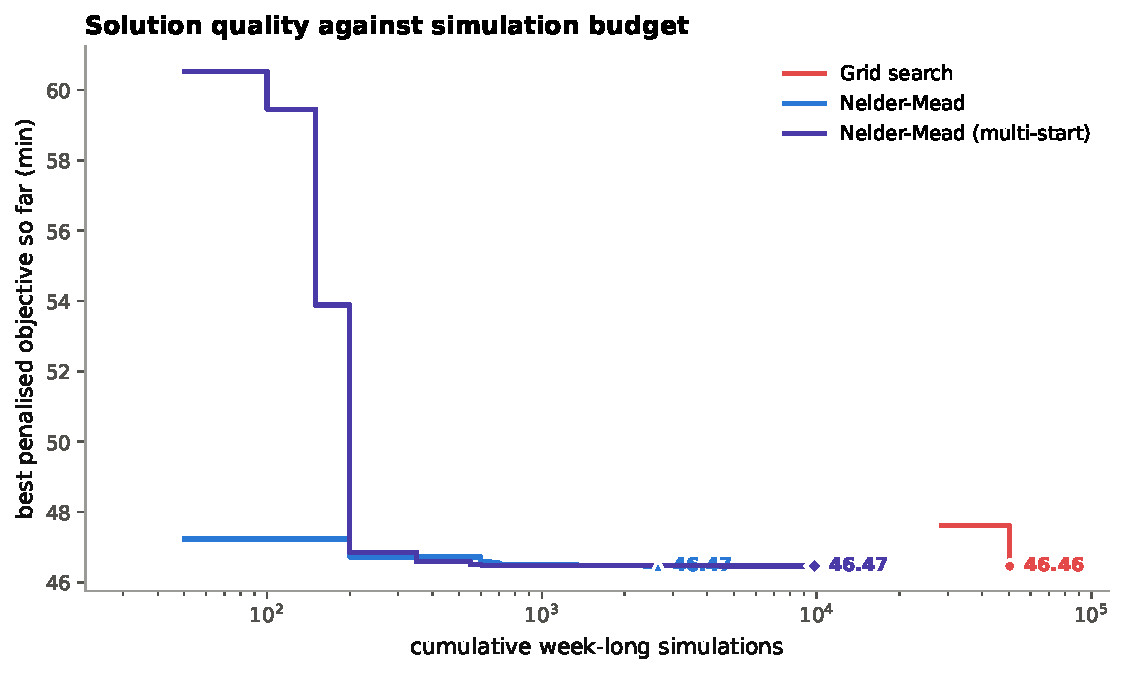
\includegraphics[width=\columnwidth]{figures/wp3_convergence.pdf}
\caption{Best objective found so far against cumulative simulation budget
         (log scale).}
\Description{Step plot of best objective versus number of simulations on a
logarithmic horizontal axis. The Nelder-Mead curves reach the same objective
level as grid search at roughly one twentieth of the budget.}
\label{fig:conv}
\end{figure}

This experiment also produced an unanticipated finding. Under the $95\%$
constraint the optimum moves to a much larger $k_2$, and the paper's published
$(13.1,2.1)$ becomes \emph{infeasible} on our model, reaching only $89.4\%$ on
Level IV (Table~\ref{tab:optconf}). The mechanism is transparent: with
$T_4=120$ and $k_2=2.1$, a Level IV patient is flagged urgent only after
waiting $117.9$ of their $120$ permitted minutes, which is too late to rescue
them on a system as congested as ours. This is the strongest argument in this
work for re-tuning under an explicit constraint rather than reusing published
parameters.

\begin{table}[t]
\caption{All three optima re-scored on identical replications.}
\label{tab:optconf}
\small
\begin{tabular}{@{}llrrrl@{}}
\toprule
\textbf{Setting} & $(k_1,k_2)$ & \textbf{Wait} & $SL_3$ & $SL_4$ & \textbf{Status} \\
\midrule
Nelder--Mead    & $(2.31, 8.37)$ & 44.18 & 95.42\% & 95.64\% & feasible \\
Grid search     & $(4.10, 8.20)$ & 44.17 & 97.73\% & 95.49\% & feasible \\
Paper           & $(13.10, 2.10)$& 44.08 & 99.99\% & 89.40\% & \textbf{infeasible} \\
\bottomrule
\end{tabular}
\end{table}

\subsection{Cost-optimal staffing}
\label{sec:resstaff}
Table~\ref{tab:staffing} prices the paper's own seven staffing scenarios under
Eq.~\eqref{eq:cost}. Where the paper can only observe that more physicians
means shorter waits --- a statement with no stopping point --- the priced
sequence has a clear interior optimum at $S_5$. A free search over all $140$
admissible rosters, with $(k_1,k_2)$ re-tuned inside each, finds a cheaper
configuration still: roster $\mathbf{(6,6,3)}$ with thresholds
$(12.20, 23.40)$. Relative to the paper's fixed $(5,5,3)$ this costs $105$
additional physician-hours per week but recovers $33$ minutes of mean waiting
per patient and cuts the SLA penalty from $4{,}913$ to $60$ cost units, for a
net weekly saving of $28{,}878$ units, or $\mathbf{20.7\%}$.

\begin{table}[t]
\caption{The base paper's seven staffing scenarios, priced under
         Eq.~\eqref{eq:cost}. Cost in arbitrary units per week.}
\label{tab:staffing}
\small
\begin{tabular}{@{}llrrrr@{}}
\toprule
& \textbf{Roster} & \textbf{Phys-h} & \textbf{Wait} & $SL_4$ & \textbf{Total} \\
\midrule
$S_0$ & (5,5,3) & 714  & 44.18 & 95.64\%  & 139{,}391 \\
$S_1$ & (5,5,4) & 777  & 35.19 & 98.53\%  & 134{,}121 \\
$S_2$ & (5,5,5) & 840  & 31.25 & 99.32\%  & 136{,}490 \\
$S_3$ & (5,6,5) & 889  & 16.34 & 99.98\%  & 124{,}942 \\
$S_4$ & (5,7,5) & 938  & 11.45 & 100.00\% & 125{,}327 \\
$S_5$ & (6,7,5) & 994  & 4.32  & 100.00\% & \best{124{,}082} \\
$S_6$ & (7,7,5) & 1050 & 2.38  & 100.00\% & 128{,}652 \\
\midrule
\multicolumn{2}{@{}l}{\textbf{Ours} (6,6,3)} & 819 & 10.97 & 99.93\% & \best{110{,}513} \\
\bottomrule
\end{tabular}
\end{table}

The joint formulation earns its complexity. Screened at one fixed threshold
pair, roster $(6,6,3)$ scores $111{,}932$; re-tuned to its own optimum
$(12.20,23.40)$ it scores $110{,}870$. More importantly the thresholds
\emph{move substantially} between rosters --- $k_2$ ranges from $11.5$ to
$25.6$ across the six refined candidates --- so holding them fixed while
varying staffing would score every alternative roster at settings chosen for a
different one.

\begin{table}[t]
\caption{Sensitivity of the staffing recommendation to the cost weights.}
\label{tab:costsens}
\small
\begin{tabular}{@{}lrrrlr@{}}
\toprule
\textbf{Scenario} & $\alpha$ & $\beta$ & $\gamma$ & \textbf{Winner} & \textbf{vs.\ (5,5,3)} \\
\midrule
Baseline              & 120 & 0.500 & 50  & (6,6,3) & $-20.7\%$ \\
Waiting $\times4$     & 120 & 2.000 & 50  & (6,7,3) & $-53.2\%$ \\
Waiting $\times\!\frac{1}{4}$ & 120 & 0.125 & 50 & (5,6,3) & $-5.2\%$ \\
Physicians $\times1.5$& 180 & 0.500 & 50  & (6,6,3) & $-12.4\%$ \\
SLA breach $\times10$ & 120 & 0.500 & 500 & (6,6,3) & $-39.5\%$ \\
\bottomrule
\end{tabular}
\end{table}

Table~\ref{tab:costsens} stress-tests the recommendation. The winning roster
\emph{changes} with the weights. We regard this not as a weakness of the method
but as the finding itself: the right staffing level genuinely depends on how a
hospital prices a patient's waiting minute against a physician's salary, so
those weights must be agreed before a roster can be set. What does not change
is that every weighting beats the paper's fixed $(5,5,3)$, by between $5.2\%$
and $53.2\%$.

\begin{figure}[t]
\centering
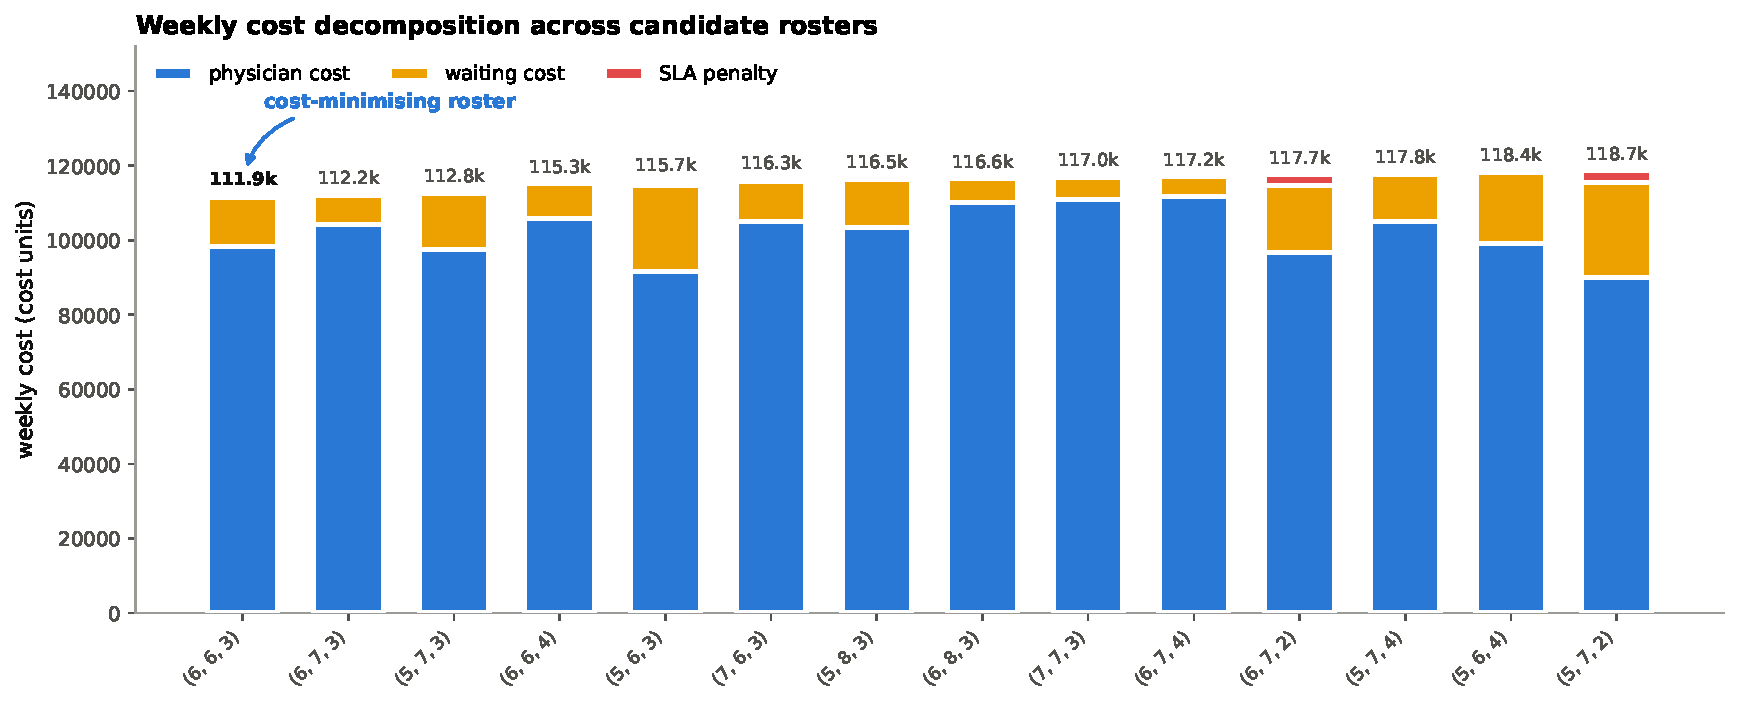
\includegraphics[width=\columnwidth]{figures/wp4_cost_decomposition.pdf}
\caption{Weekly cost decomposed into physician, waiting and SLA-penalty
         components across the best screened rosters.}
\Description{Stacked bar chart across fourteen candidate rosters. Physician
cost dominates each bar; waiting cost shrinks as staffing rises while physician
cost grows, producing a minimum total at roster six six three.}
\label{fig:cost}
\end{figure}

\subsection{Variance reduction}
Table~\ref{tab:crn} reports the effect of CRN on every pairwise comparison.
The induced correlations range from $+0.996$ to $+0.9996$, against
$\approx0$ under independent streams, and the median variance removed is
$\mathbf{98.95\%}$, a median efficiency gain of $\mathbf{95.8\times}$.
Confidence intervals on the mean difference narrow by factors of $4$ to $40$.

\begin{table}[t]
\caption{Variance of the pairwise difference in mean waiting time, with and
         without common random numbers; $100$ replications per arm.}
\label{tab:crn}
\small
\begin{tabular}{@{}lrrrr@{}}
\toprule
\textbf{Comparison} & \textbf{Var ind.} & \textbf{Var CRN} & \textbf{Removed} & \textbf{Gain} \\
\midrule
IFP vs.\ ALT     & 241.34 & 12.44 & 94.85\% & 19.4$\times$ \\
IFP vs.\ SBP     & 330.48 & 6.12  & 98.15\% & 54.0$\times$ \\
IFP vs.\ WSEPT   & 288.20 & 13.16 & 95.43\% & 21.9$\times$ \\
IFP vs.\ Gc$\mu$ & 216.19 & 8.50  & 96.07\% & 25.4$\times$ \\
ALT vs.\ SBP     & 220.77 & 2.15  & 99.03\% & 102.9$\times$ \\
ALT vs.\ WSEPT   & 191.64 & 0.11  & 99.94\% & 1789.3$\times$ \\
ALT vs.\ Gc$\mu$ & 223.75 & 0.46  & 99.79\% & 485.4$\times$ \\
SBP vs.\ WSEPT   & 198.04 & 2.23  & 98.87\% & 88.7$\times$ \\
SBP vs.\ Gc$\mu$ & 268.97 & 1.03  & 99.62\% & 261.8$\times$ \\
WSEPT vs.\ Gc$\mu$& 215.27 & 0.59 & 99.72\% & 362.7$\times$ \\
\midrule
\multicolumn{3}{@{}l}{\textbf{Median}} & \best{98.95\%} & \best{95.8$\times$} \\
\bottomrule
\end{tabular}
\end{table}

Two properties deserve emphasis. First, CRN is not a bias: the per-policy means
and standard deviations agree between the two arms within sampling error, as
theory requires, since only the joint distribution changes. Second, it changes
conclusions --- several comparisons that fail to reach the Bonferroni threshold
under independent streams are decisive under CRN. Where the arms disagree, CRN
is the arm to believe, because it estimates the same quantity with lower
variance.

We are careful not to over-claim. A $95.8\times$ efficiency gain does not mean
one replication suffices: the ratio is itself estimated, and a $t$-interval
needs adequate degrees of freedom. The defensible practical reading is that
$20$--$30$ CRN replications give comparisons at least as sharp as the base
paper's $100$ independent ones --- a $3$--$5\times$ saving that can safely be
taken.

\begin{figure}[t]
\centering
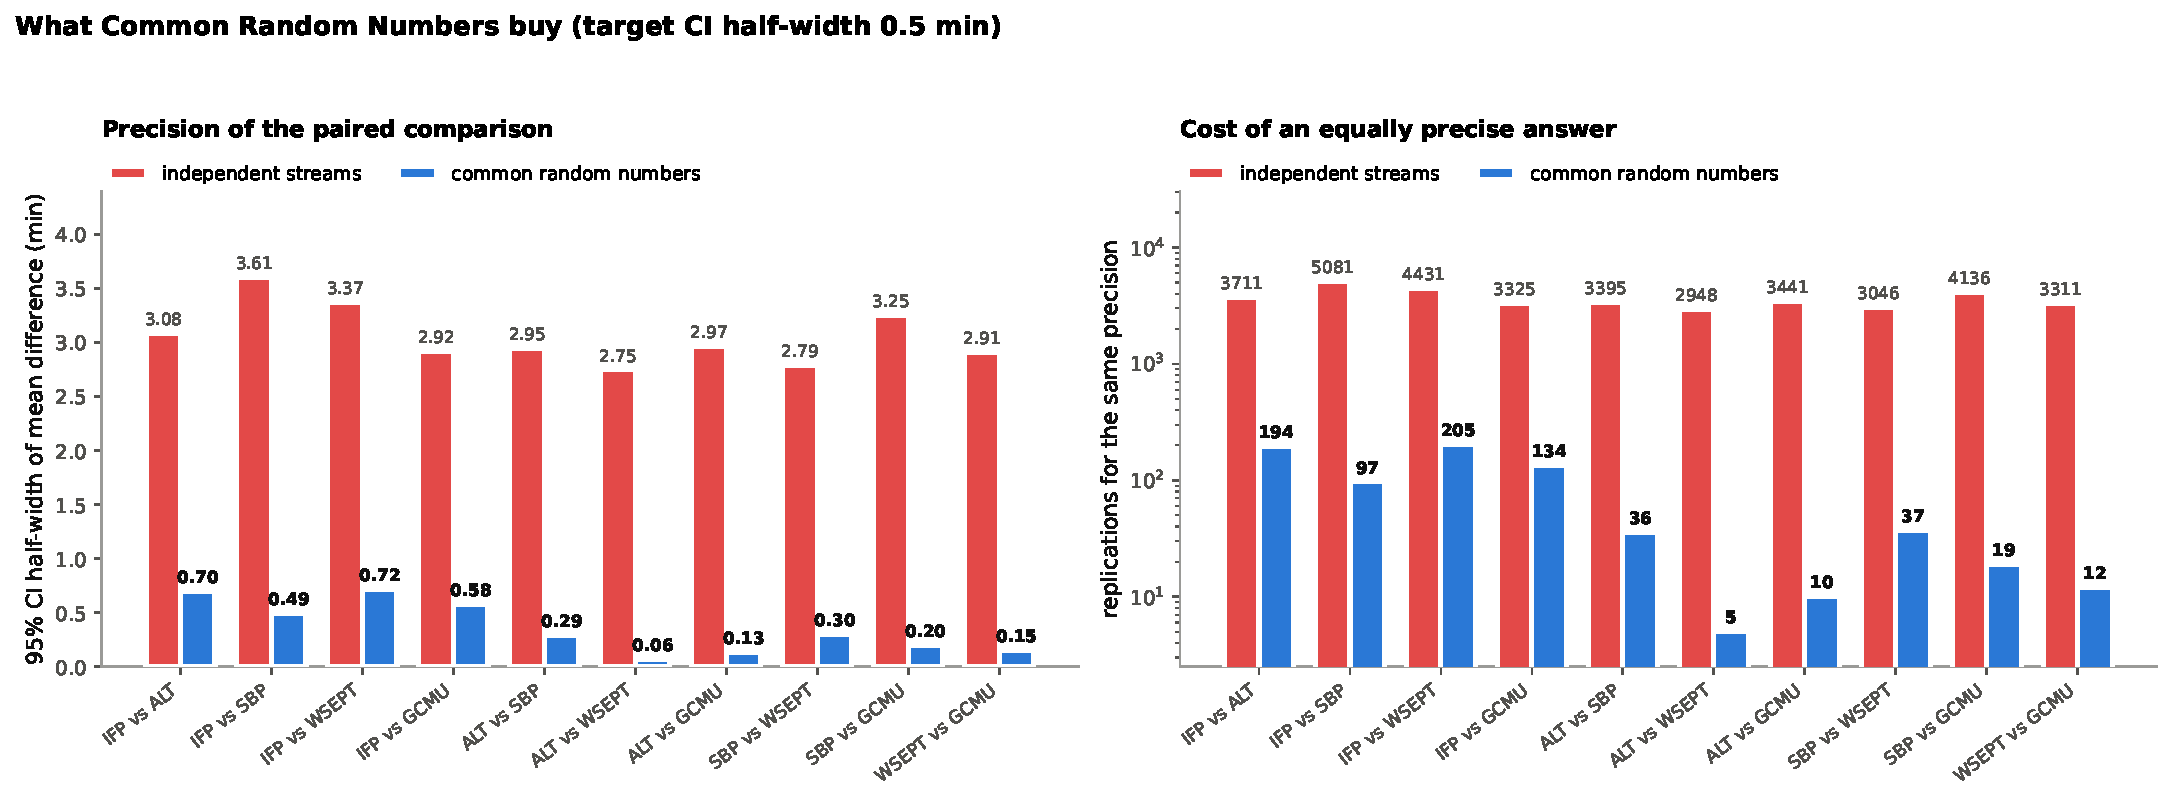
\includegraphics[width=\columnwidth]{figures/wp5_crn_variance_reduction.pdf}
\caption{Left: 95\% confidence-interval half-width on each pairwise difference.
         Right: replications needed for $\pm0.5$~min precision (log scale).}
\Description{Two grouped bar charts over ten policy pairs. In both, the common
random numbers bars are far shorter than the independent stream bars; the
right panel shows thousands of replications reduced to tens.}
\label{fig:crn}
\end{figure}

\subsection{Robustness}
We reproduce all three of the base paper's sensitivity studies and extend them
to the added policies. Scaling every arrival rate by $-15\%$ to $+15\%$
(Figure~\ref{fig:arr}) drives $\rho$ from $0.739$ to $1.000$; the policies are
nearly interchangeable under light load and diverge sharply as the system
saturates, the policy spread growing from $1.6$ to $53$~min. Across the seven
staffing scenarios (Figure~\ref{fig:staff}) waits fall with clear diminishing
returns and the \emph{choice} of policy matters most exactly when physicians
are scarce, the spread falling from $10.1$~min at $S_0$ to $0.06$~min at $S_6$.
Finally, replacing the truncated exponential service times with truncated
lognormals of the same nominal means raises all waits by $44$--$54\%$ through
the heavier right tail, but leaves the ranking \emph{identical}, confirming
that the comparative conclusions are not an artefact of the distributional
assumption. All three findings match the base paper.

\begin{figure}[t]
\centering
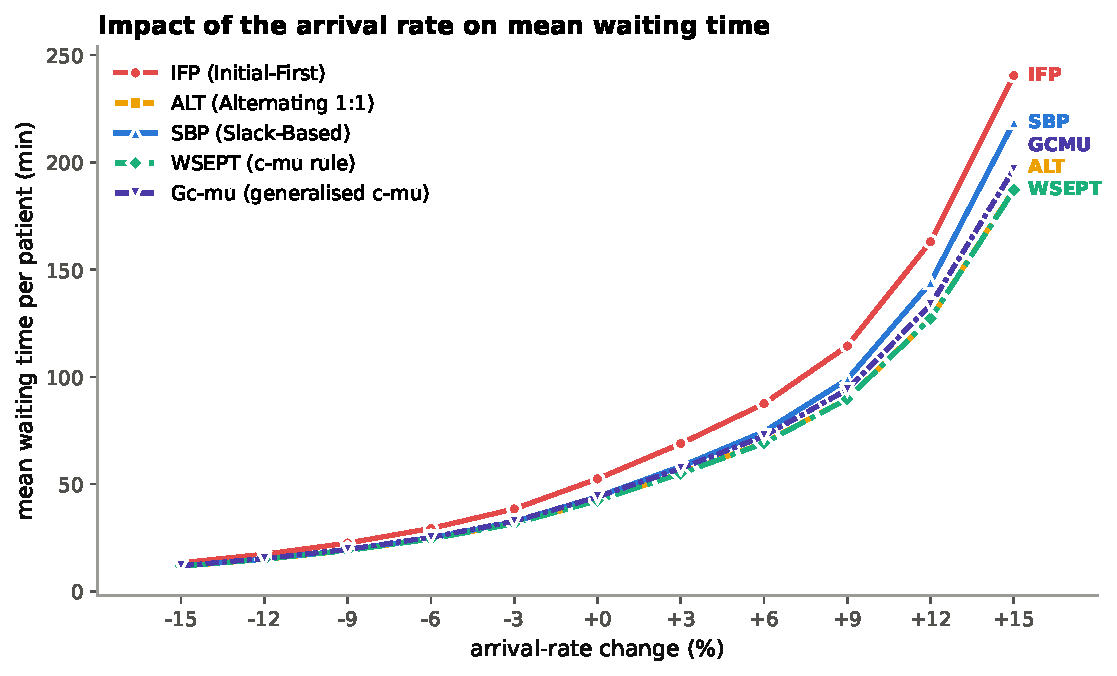
\includegraphics[width=\columnwidth]{figures/sens_arrival_rate.pdf}
\caption{Impact of the arrival rate on mean waiting time, all five policies.}
\Description{Five rising curves of mean waiting time against arrival rate
change from minus fifteen to plus fifteen percent. All curves coincide at the
left and fan out steeply at the right, with IFP highest throughout.}
\label{fig:arr}
\end{figure}

\begin{figure}[t]
\centering
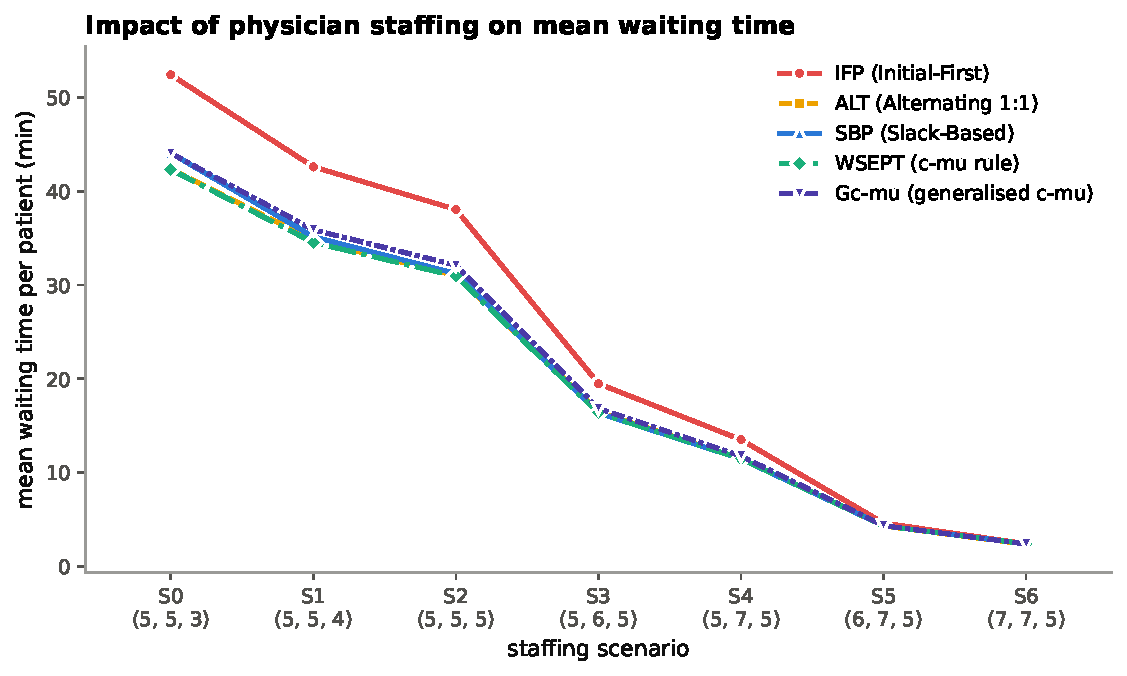
\includegraphics[width=\columnwidth]{figures/sens_staffing.pdf}
\caption{Impact of physician staffing on mean waiting time across the base
         paper's seven scenarios.}
\Description{Five descending curves of mean waiting time across staffing
scenarios S0 to S6. The curves are separated at S0 and converge to almost the
same value by S6.}
\label{fig:staff}
\end{figure}

\subsection{Threats to validity}
Three limitations bound the claims above. \emph{Construct}: the base paper's
dataset is unavailable, so we calibrate to published summary statistics only;
the $12$--$25\%$ level mismatch is the visible consequence, and only relative
conclusions should be carried forward. \emph{Internal}: five parameters are our
choice; four are swept or stress-tested, and the fifth ($SL^{\min}$) is
reported alongside both raw service levels so a different threshold can be
applied by inspection. \emph{External}: the model is one ED with one triage
system; the c$\mu$ optimality guarantee is weakened by re-entrant flow, and the
cost weights are illustrative rather than institutional.

%% ======================================================================
\section{Conclusion and Future Work}

We rebuilt the discrete-event model of Lv et al.~\cite{lv2026des} from its
published parameters alone and validated it against every KPI the paper
reports. All six structural findings reproduce, including the
equipment-utilisation table to within $0.5$ percentage points and all three
sensitivity-analysis conclusions; absolute waiting times run $12$--$25\%$
higher, which we trace to the implied load $\rho\approx0.87$ and report rather
than tune away.

Four extensions follow. A c$\mu$-based policy, provably optimal for a stated
delay-cost objective, attains the lowest holding cost ($-50\%$ against IFP) and
the lowest raw mean wait. A hand-implemented Nelder--Mead simplex with an
exterior penalty reaches the lattice optimum to within $0.006$~min using
$19\times$ fewer week-long simulations. An explicit cost model identifies
roster $(6,6,3)$ with re-tuned thresholds as $20.7\%$ cheaper per week than the
paper's fixed $(5,5,3)$, with the winner's sensitivity to the cost weights
reported as a finding in its own right. Exact common random numbers remove
$98.9\%$ of the variance of every pairwise comparison.

The single most consequential result is negative: on our model the base paper's
own published thresholds $(13.1, 2.1)$ violate a $95\%$ Level IV service-level
constraint, because $k_2 = 2.1$ defers intervention to minute $117.9$ of $120$.
Constrained re-tuning restores feasibility and yields the only tuned policy
that a hospital could adopt. Published scheduling parameters are properties of
the system they were fitted to, not transferable constants.

Future work follows three lines. The c$\mu$ guarantee should be re-derived for
the re-entrant, time-varying setting actually present here, where only
asymptotic results are currently available. The optimiser could be extended to
higher-dimensional decision vectors --- per-shift thresholds, or thresholds that
adapt to the observed queue state --- where the advantage over lattice search
grows combinatorially and where the base paper itself suggests reinforcement
learning. Finally, the cost model invites a formal stochastic-programming
treatment in which the roster is a first-stage decision and the thresholds a
recourse decision, which would replace our two-stage screening heuristic with a
principled decomposition.

%% ======================================================================
\begin{acks}
We thank the course instructors of CSE~402 for guidance on scope and
methodology. All simulation code, generated result tables, figures and a
complete provenance log recording the exact command behind every artefact are
available at \url{\REPOURL}.
\end{acks}

\bibliographystyle{ACM-Reference-Format}
\bibliography{references}

\end{document}
